%
% Documento: Abordagem e modelagem do Problema
%

\chapter{Abordagem e Modelagem do Problema}
\label{chap:abordagememdelo}
Este trabalho tem como intuito modelar uma malha de controle, que conduza uma frota de robôs dado um alvo de posição \emph{x,y} no espaço, à circundar esse alvo à uma distância \emph{R}. E modelar uma malha de controle, responsável pelo controle de formação da tropa de robôs, em que devido à falha de um ou mais robôs, a tropa consiga se reestruturar para cobrir melhor a circunferência ao redor do alvo. Ou seja, caso um ou mais robôs saiam da rede, a frota ira se reajustar para que cada robô tenha a mesma distância entre si e assim, não fique uma grande parte da fronteira sem cobertura, como demostrado na \autoref{sistema} abaixo. Que representa uma frota de quatro robôs andando ao redor do alvo, quando então, um dos robôs falha. E o sistema se reajusta para adaptar-se à rede de apenas três robôs.

\begin{figure}[!htb]
	\centering
	\caption{Modelagem do Sistema}
	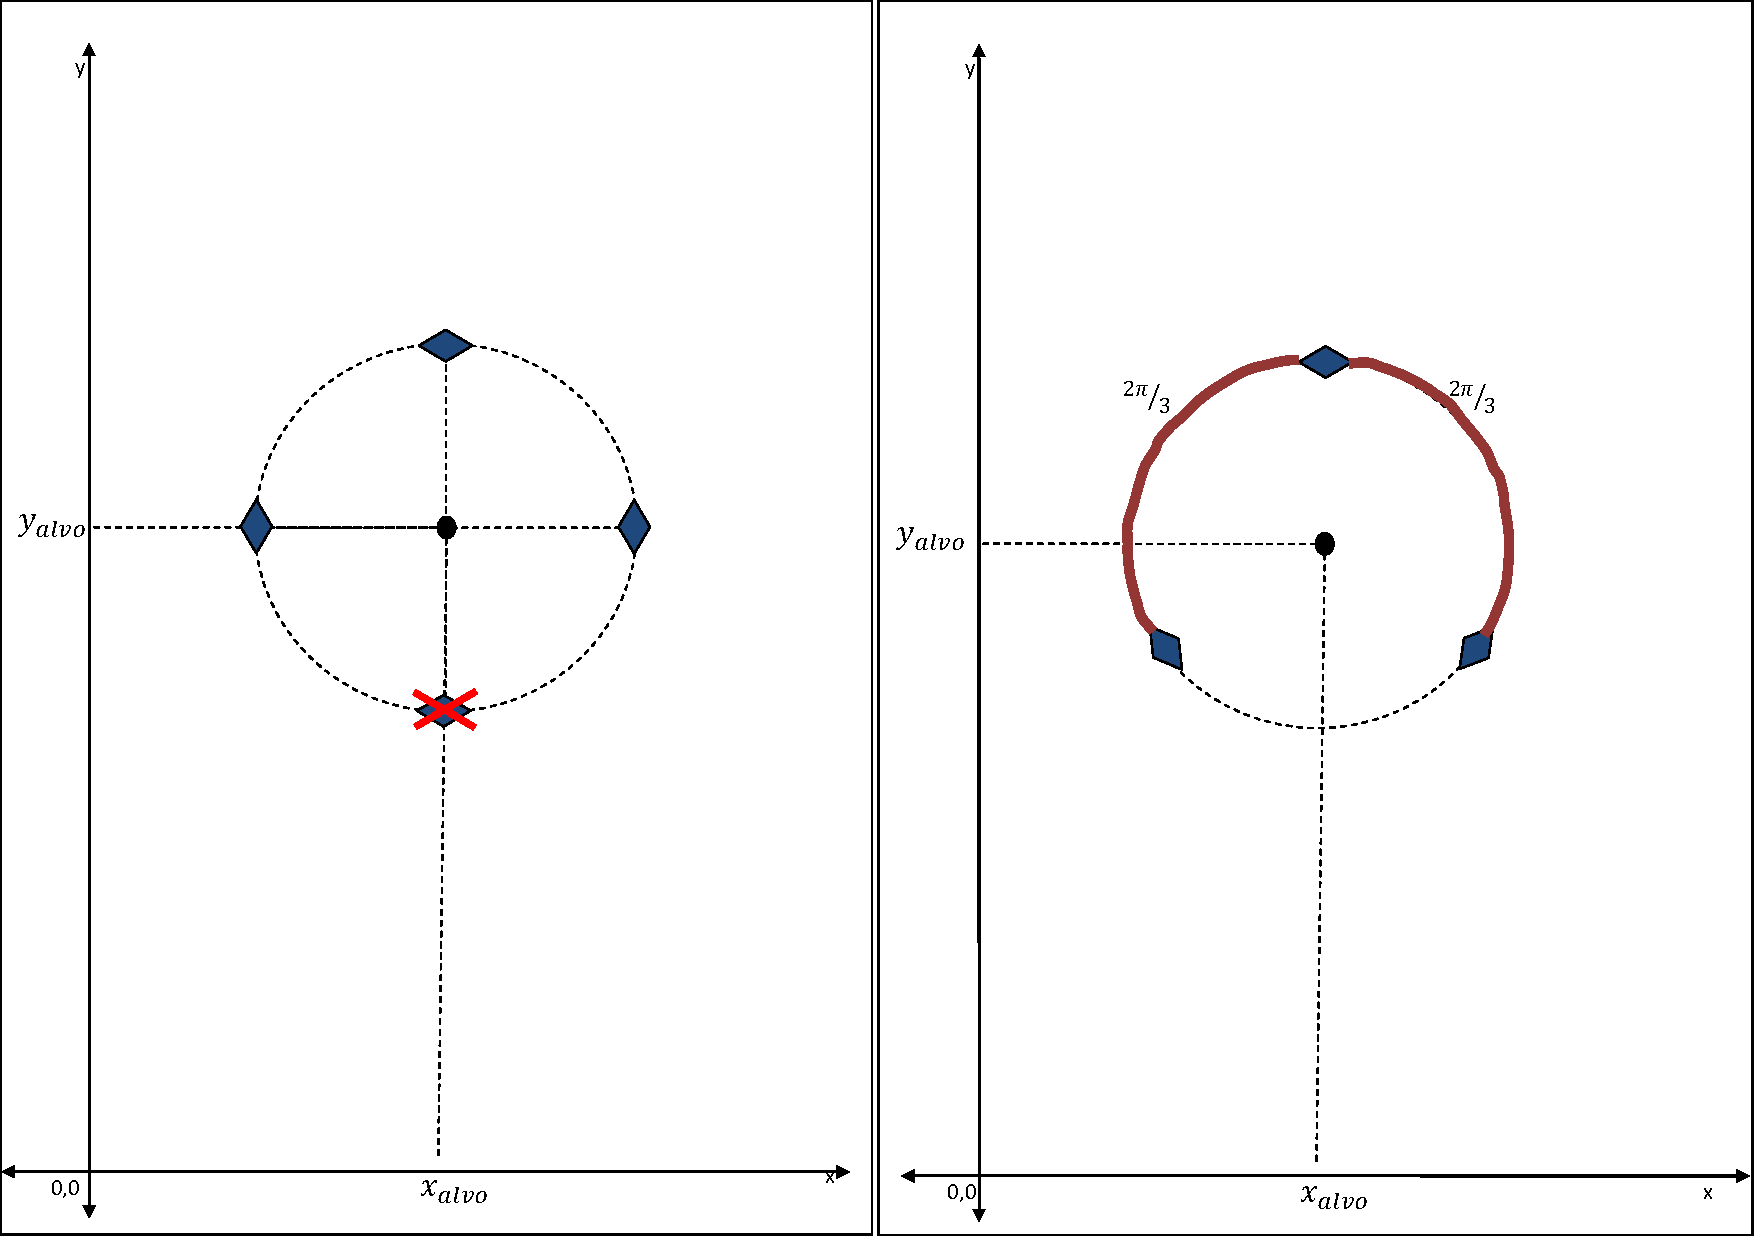
\includegraphics[width=1.0\textwidth]{./04-figuras/sistema}
	\label{fig:sistema}
\end{figure}

Neste capítulo faremos um detalhamento do funcionamento do sistema como um todo e a modelagem escolhida para abordar o problema. Primeiramente, iremos utilizar uma abordagem já mencionada anteriormente, que é o controle em cascata, utilizada para modularizar o problema e assim, tornar mais simples a implementação. Serão três malhas de controle: A primeira e mais interna será responsável pelo controle da velocidade angular de cada roda, para se chegar à posição \emph{x,y} desejada. Esta malha estará presente em cada um dos robôs da frota que estarão à circular o alvo. A segunda, malha intermediária, será responsável para que cada robô chegue à um determinado ponto \emph{x,y} no espaço, portanto, será responsável por corrigir o posicionamento do robô. Esta malha também estará presente em cada robô que circundar o alvo. A terceira malha, e portanto, a mais externa é responsável pela coordenação da frota, dizendo à cada robô o ponto \emph{x,y}, onde o mesmo deve ficar.

Existem diversas maneiras de se implementar um sistema como este, tanto do ponto de vista do sistema distribuído e sua rede de comunicação, quanto do ponto de vista de controle e realimentação das malhas. Neste trabalho, começaremos abordando o sistema de controle, com as duas malhas mais internas para então, abordar o sistema como um sistema de controle distribuído.
 
\section{Malha de Controle 1: Velocidade Angular das Rodas}
\label{sec:malha1 } 
Como já dito anteriormente neste trabalho, este sistema de controle consiste em um controle de três malhas, e agora abordaremos sobre a primeira malha. A primeira malha controla os motores para atingir a velocidade angular desejada ($ \omega _{d} $). Ou seja, deseja-se circular o alvo em um período de \emph{T} segundos, a malha de controle de velocidade vai receber a velocidade angular desejada ($ \omega _{d} $), que é uma derivação do período de circulação desejado, como mostrado na equação abaixo:
\begin{equation}
\omega = \dfrac{2\pi}{T}
\label{eq:velocangular}
\end{equation}

A partir daí o módulo calcula velocidade angular desejada de cada roda ($ \omega _{dr} $: velocidade angular desejada da roda direita, $ \omega _{dl} $: velocidade angular desejada da roda esquerda), a partir das equações abaixo:
\begin{equation}
\omega_{dr} = \dfrac{2v + \omega_{d}L}{2r_{p}}	
\label{eq:velocangulardireita}
\end{equation} 

\begin{equation}
\omega_{dl} = \dfrac{2v - \omega_{d}L}{2r_{p}}	
\label{eq:velocangularesquerda}
\end{equation} 

,onde $v \rightarrow$ velocidade linear (m/s) desejada do robô 
      $r_{p} \rightarrow$ raio do pneu (m)
	  $L \rightarrow$ tamanho do eixo do robô (m)

\begin{equation}
\dot{x} = v\cos(\theta) 
\label{eq:posiçãox}
\end{equation}
\begin{equation}
\dot{y} = v\sin(\theta)
\label{eq:posiçãoy}
\end{equation}
\begin{equation}
\dot{\theta} = \omega
\label{eq:posiçãotheta}
\end{equation}




\begin{figure}[!htb]
	\centering
	\caption{Primeira malha de Controle do Sistema - Controle da velocidade angular}
	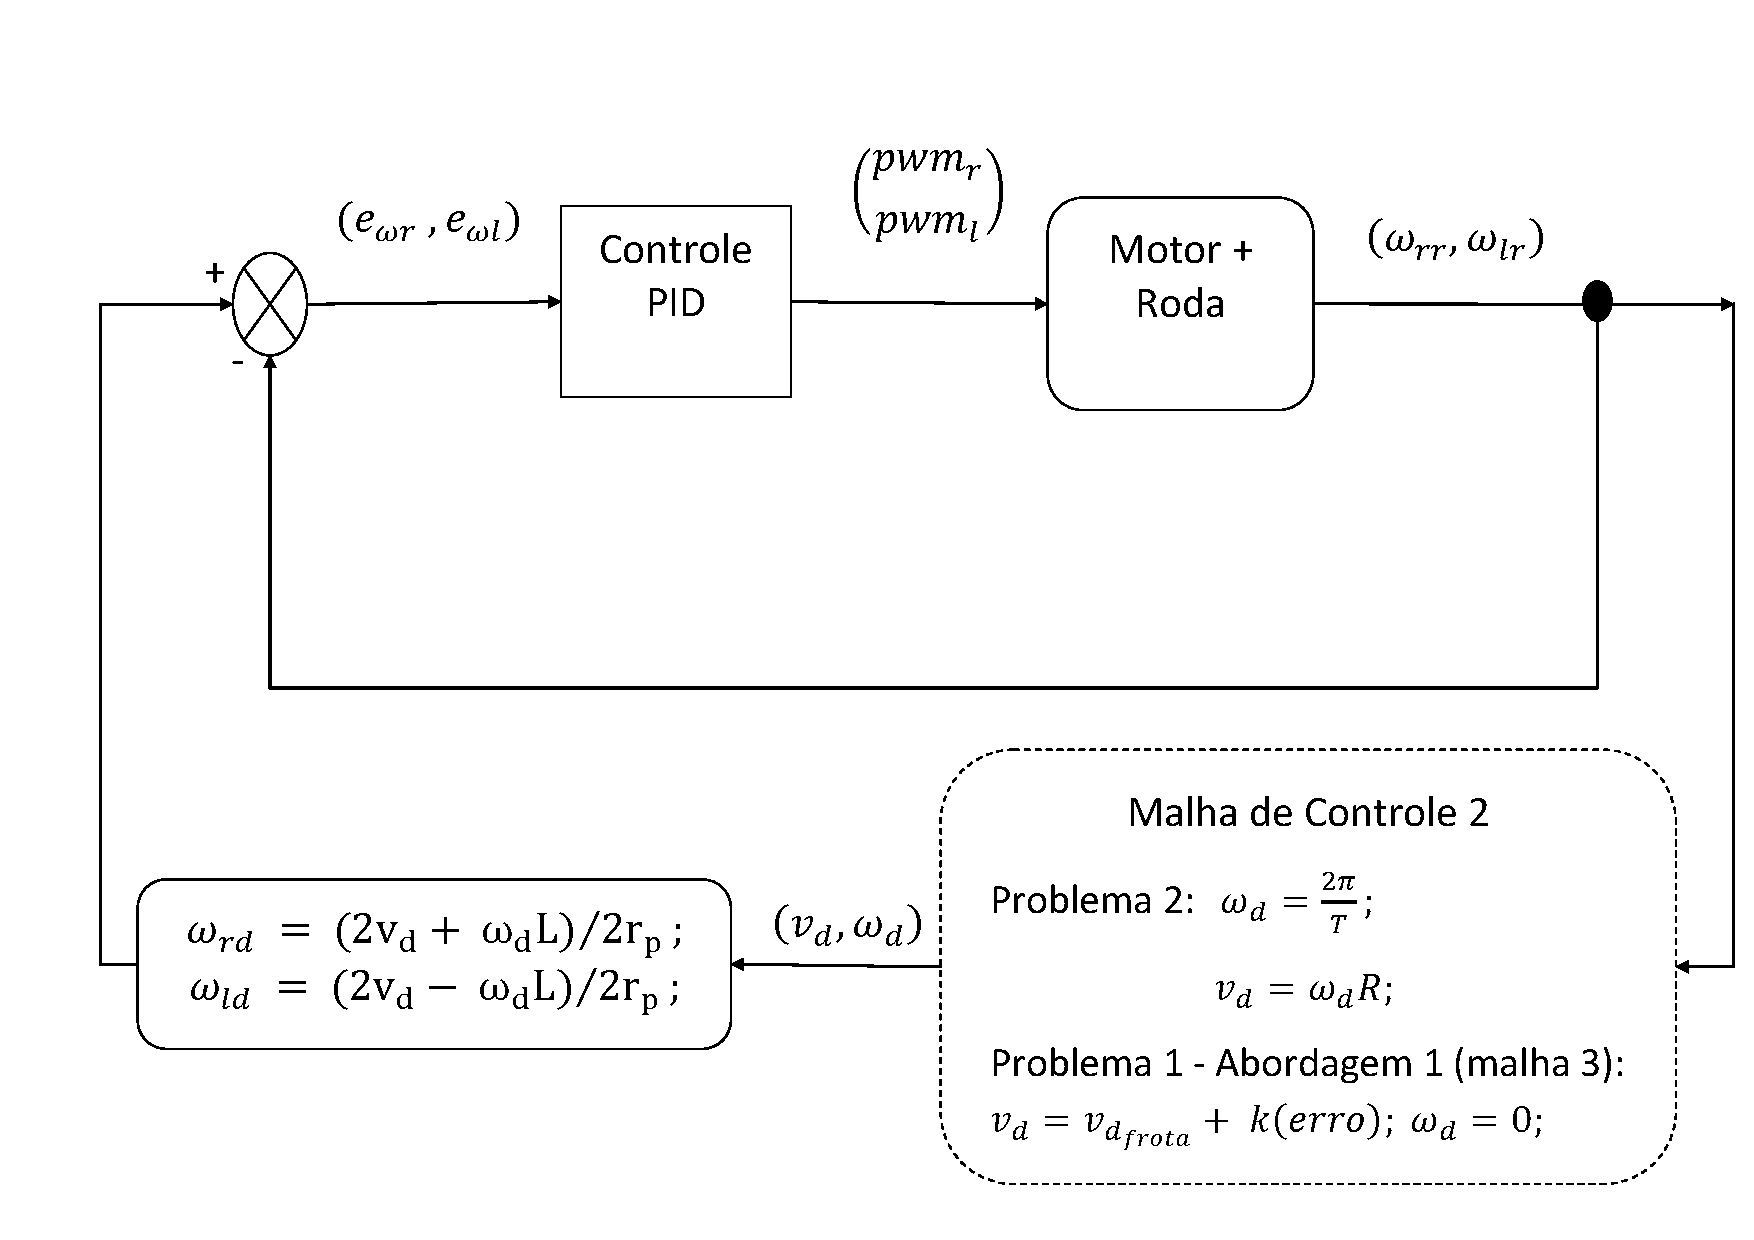
\includegraphics[width=1.0\textwidth]{./04-figuras/malha1}
	\
	\label{fig:malha1}
\end{figure}

